\section{Method}
\label{4}
\subsection{Overview}
\label{4.1}

Given the CLU objectives in Section~\ref{1.0}, we propose Bi-Directional LoRA (BID-LoRA). The name reflects the framework's dual operational direction: one direction incorporates new knowledge Eq.~\ref{Eq:3c}, while the other removes unwanted knowledge Eq.~\ref{Eq:3a}, all while preserving retained knowledge Eq.~\ref{Eq:3b}. \textcolor{red}{The ``Bi-Directional'' thus refers to these two opposing knowledge operations (learning and unlearning), not to the number of adapters. Three adapters (retain, new, forget) are the implementation mechanism that realizes this bidirectional design.}

BID-LoRA employs three dedicated LoRA adapters each with a separate pathway for retention, acquisition, and forgetting along with corresponding loss functions. This pathway separation prevents gradient interference between competing objectives. To maintain parameter efficiency, only lightweight adapters in attention layers are trained while the backbone remains frozen, following evidence that smaller network alterations reduce catastrophic forgetting~\cite{zhao2024continual}. Additionally, a replay buffer $D_r$ (see Section~\ref{3}) mitigates catastrophic forgetting of retained classes. Section~\ref{4.3} details the loss functions.

\subsection{BID-LoRA}
\label{4.2}

\medskip
\noindent
\textit{LoRA-based Model Tuning:}
We employ LoRA-based fine-tuning on attention layers as shown in Fig~\ref{fig:BIDlora_pipeline}, which encode significant knowledge in transformer architectures. A standard linear layer computes $h = Wx$, where $x \in \mathbb{R}^{k}$ is the input vector, $h \in \mathbb{R}^{d}$ is the output vector, and $W \in \mathbb{R}^{d \times k}$ is the weight matrix. LoRA introduces a low-rank update $\Delta W = BA$, where $B \in \mathbb{R}^{d \times r}$ and $A \in \mathbb{R}^{r \times k}$ are low-rank matrices, yielding $h = Wx + \mathcal{S}(BAx)$ with scaling factor $\mathcal{S}$.

\begin{figure}[!htbp]
    \centering
    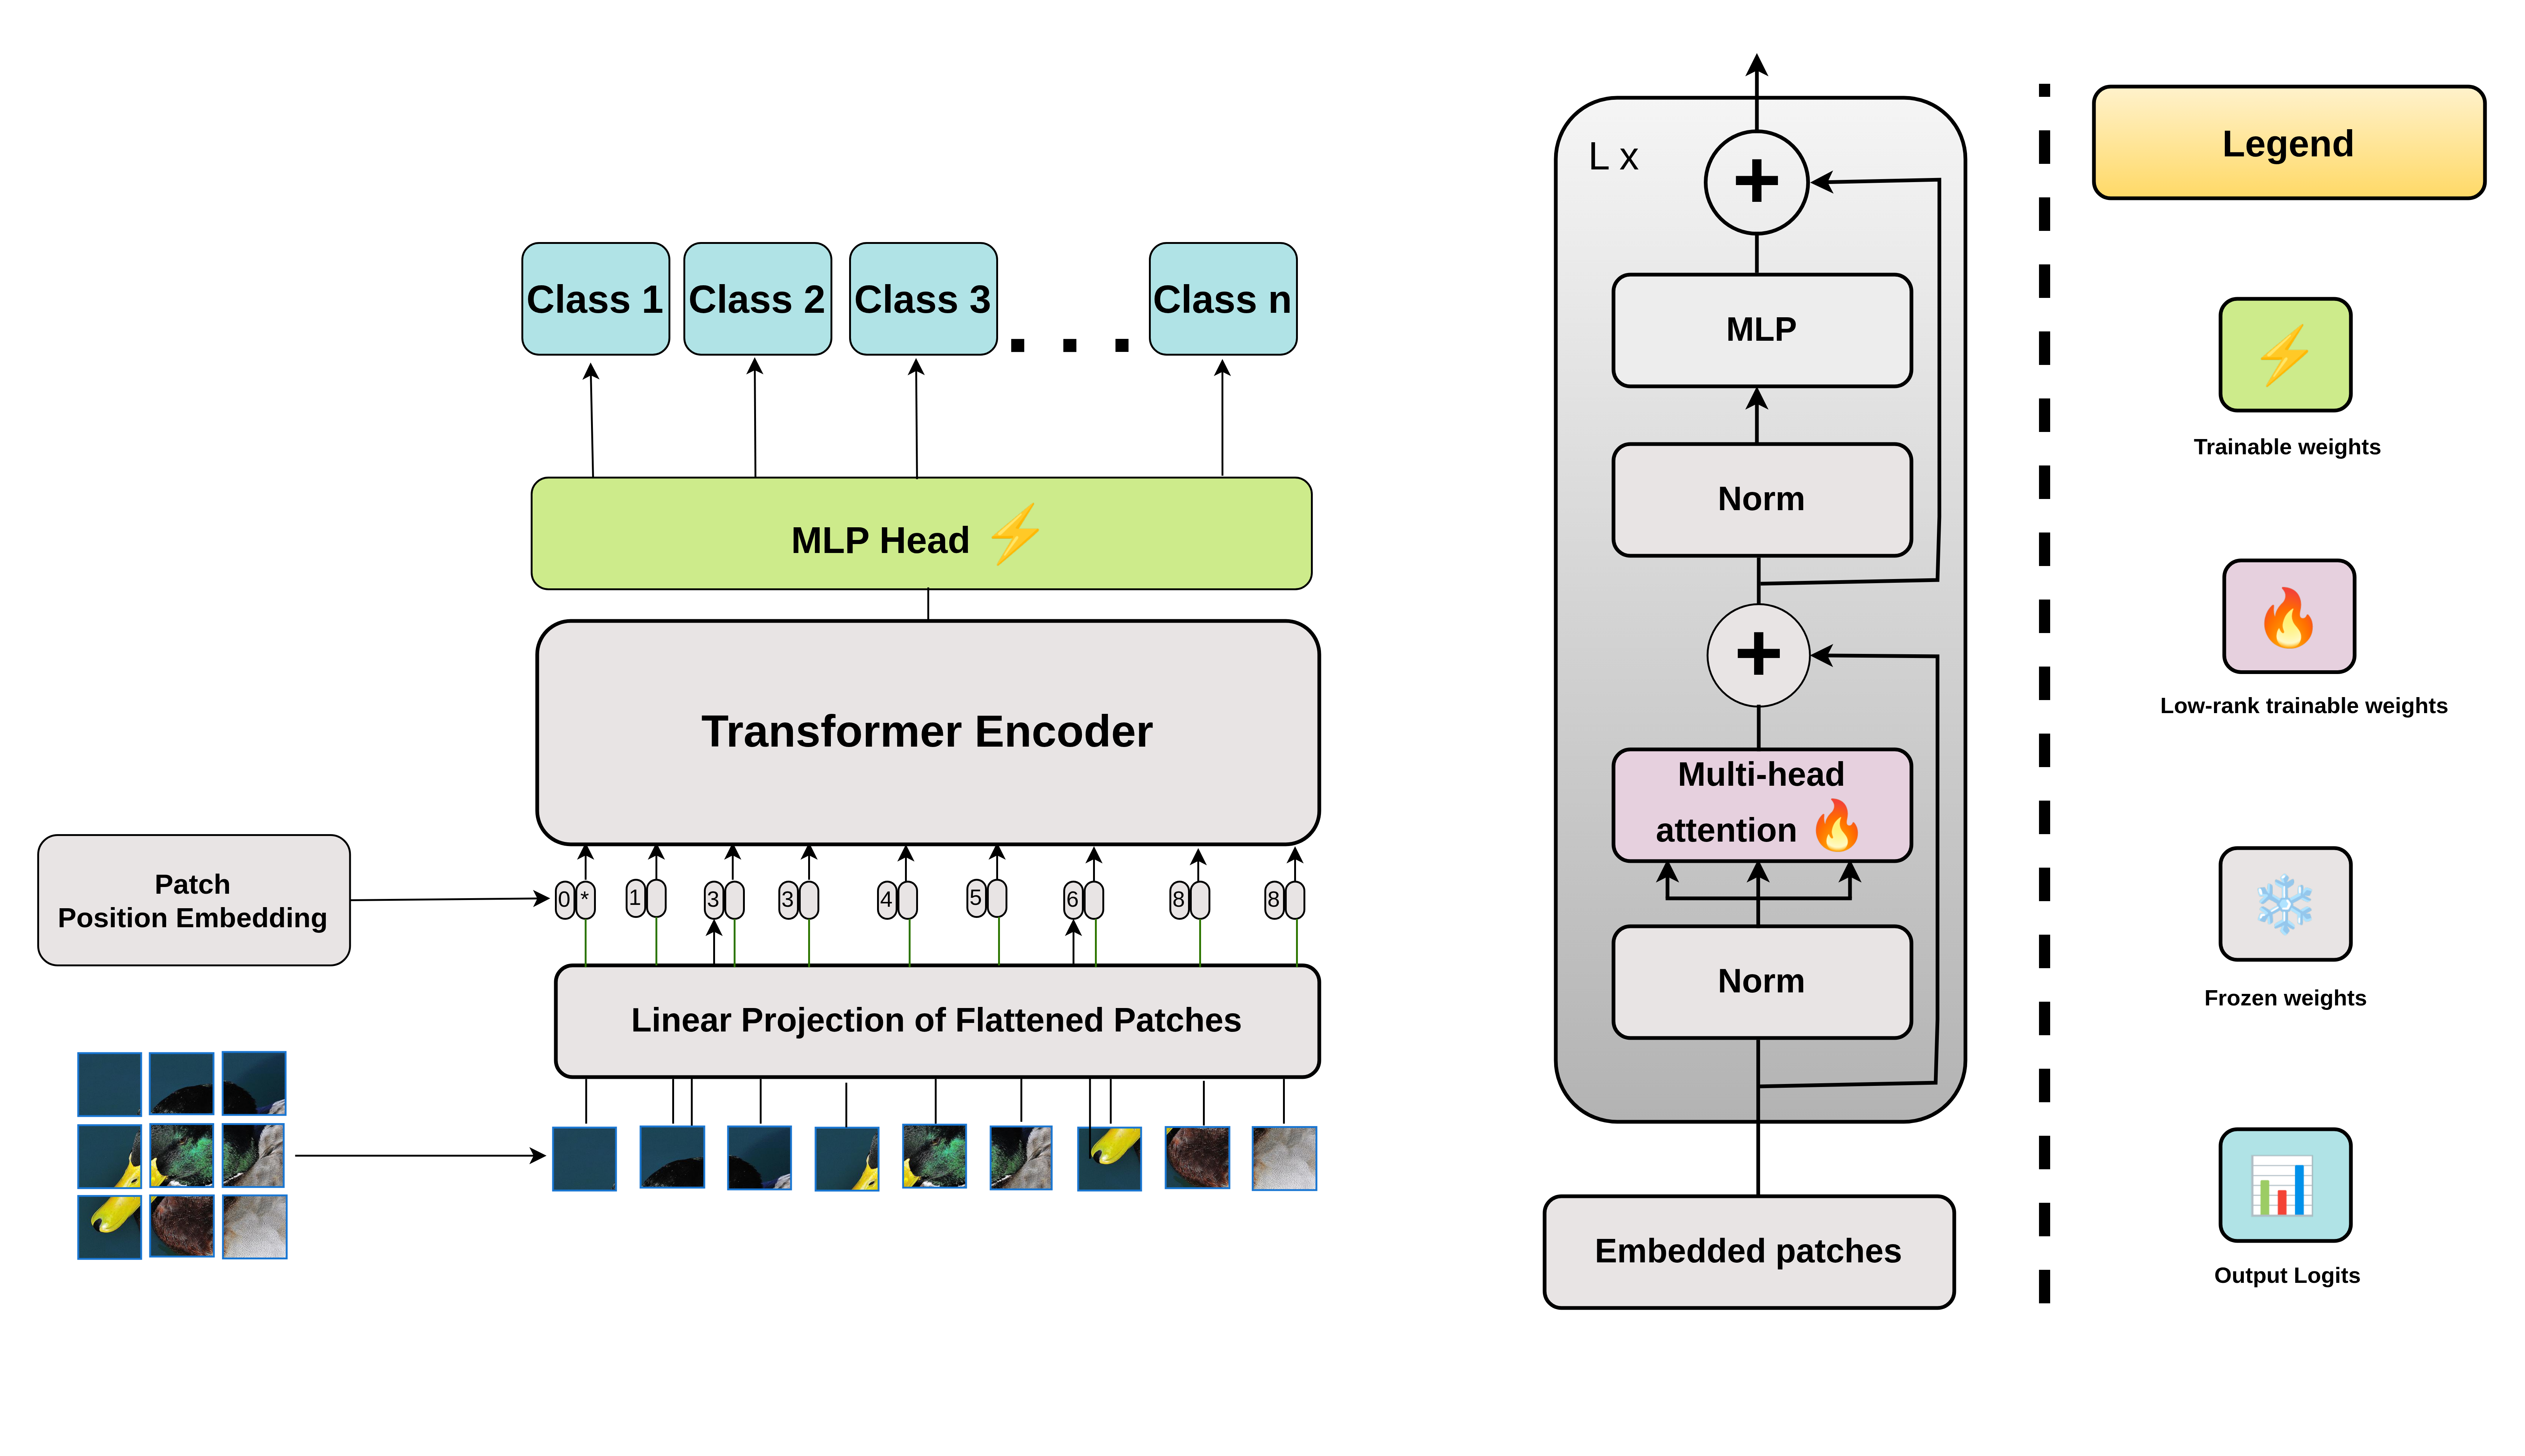
\includegraphics[width=0.75\textwidth]{images/Lora_Placement.png}
    \caption{LoRA placement in BID-LoRA at Attention Modules}
    \label{fig:BIDlora_pipeline}
\end{figure}

However, standard LoRA in CLU settings suffers from knowledge leakage gradual degradation of retained knowledge across successive steps (see Section~\ref{8.2}). \textcolor{red}{This is a direct consequence of shared parameterization: a single adapter's low-rank subspace $(B, A)$ must simultaneously satisfy retention, acquisition, and forgetting objectives within one cycle, whose gradients can point in conflicting directions within that same subspace, forcing each update to be a compromise between competing goals. Dedicating a disjoint low-rank subspace to each objective removes this conflict by construction: within a cycle, no objective's gradient can act on another's parameters, since they occupy physically separate matrices rather than a shared one. Each cycle's three adapters are freshly initialized and merged into the frozen base weights $W$ at the end of that cycle (Algorithm~\ref{alg:bidlora}); $W$, not the adapters, is therefore the only state carried across cycles, so a class's role transitioning from new to retained to forgotten over time is mediated by $W$'s accumulated updates, not by any adapter being reused across roles.}

\medskip
\noindent
\textit{Pathway Separation:}
To address cumulative knowledge drift, i.e., knowledge leakage, we dedicate distinct adapters to each objective: $W_f = B_{f}A_{f}$ for forgetting, $W_{\text{\textit{ret}}} = B_{\text{\textit{ret}}}A_{\text{\textit{ret}}}$ for retention, and $W_{\text{\textit{new}}} = B_{\text{\textit{new}}}A_{\text{\textit{new}}}$ for learning new classes. Critically, $W_f$ learns weights that \textit{nullify} forget-class knowledge, $W_{\text{\textit{new}}}$ acquires new knowledge, while $W_{\text{\textit{ret}}}$ preserves retained knowledge to counteract the knowledge leakage caused by both forget and new adapters. After sufficient training, adapters merge into the base weights $W$ as shown in Fig~\ref{fig:path_way_sepration}

\begin{equation}
h = Wx + \mathcal{S}\left(B_{\text{\textit{ret}}}A_{\text{\textit{ret}}} + B_{\text{\textit{new}}}A_{\text{\textit{new}}} + B_{\text{\textit{f}}}A_{\text{\textit{f}}}\right)x
\label{eq:merge}
\end{equation}
where $W \in \mathbb{R}^{d \times k}$ is frozen, and adapter consists of matrices $B_f,B_\text{\textit{ret}},B_\text{\textit{new}} \in \mathbb{R}^{d \times r}$ and $A_f,A_\text{\textit{ret}},A_\text{\textit{new}} \in \mathbb{R}^{r \times k}$ that serve their designated function. This separation provides two benefits: (1) drift in one adapter does not corrupt others, and (2) \textcolor{red}{each adapter's \textit{parameters} are updated only by its designated objective, without parameter interference from the other two pathways (gradients are still computed against the shared activation $h$, but only the designated adapter's weights are modified)}. Adapters merge at inference, preserving efficiency. We empirically validate pathway specialization in Section~\ref{7.4}.

\subsection{Loss Function}
\label{4.3}

In this section, we present the loss functions which are designed to balance forgetting, retention, and new knowledge acquisition in our continual adaptation framework.

\medskip
\noindent
\textit{Selective Forget Loss:}
Existing unlearning methods suffer from strong unlearning signals that degrade retention knowledge, resulting in improper forgetting. To address this, we propose \textit{Escape Unlearning}, a passive approach that pushes forget-class embeddings to an ``escape'' point maximally distant from all retain-class centroids, creating irreversible information loss. First, we compute the centroid of each class as:

\begin{figure}[!htbp]
    \centering
    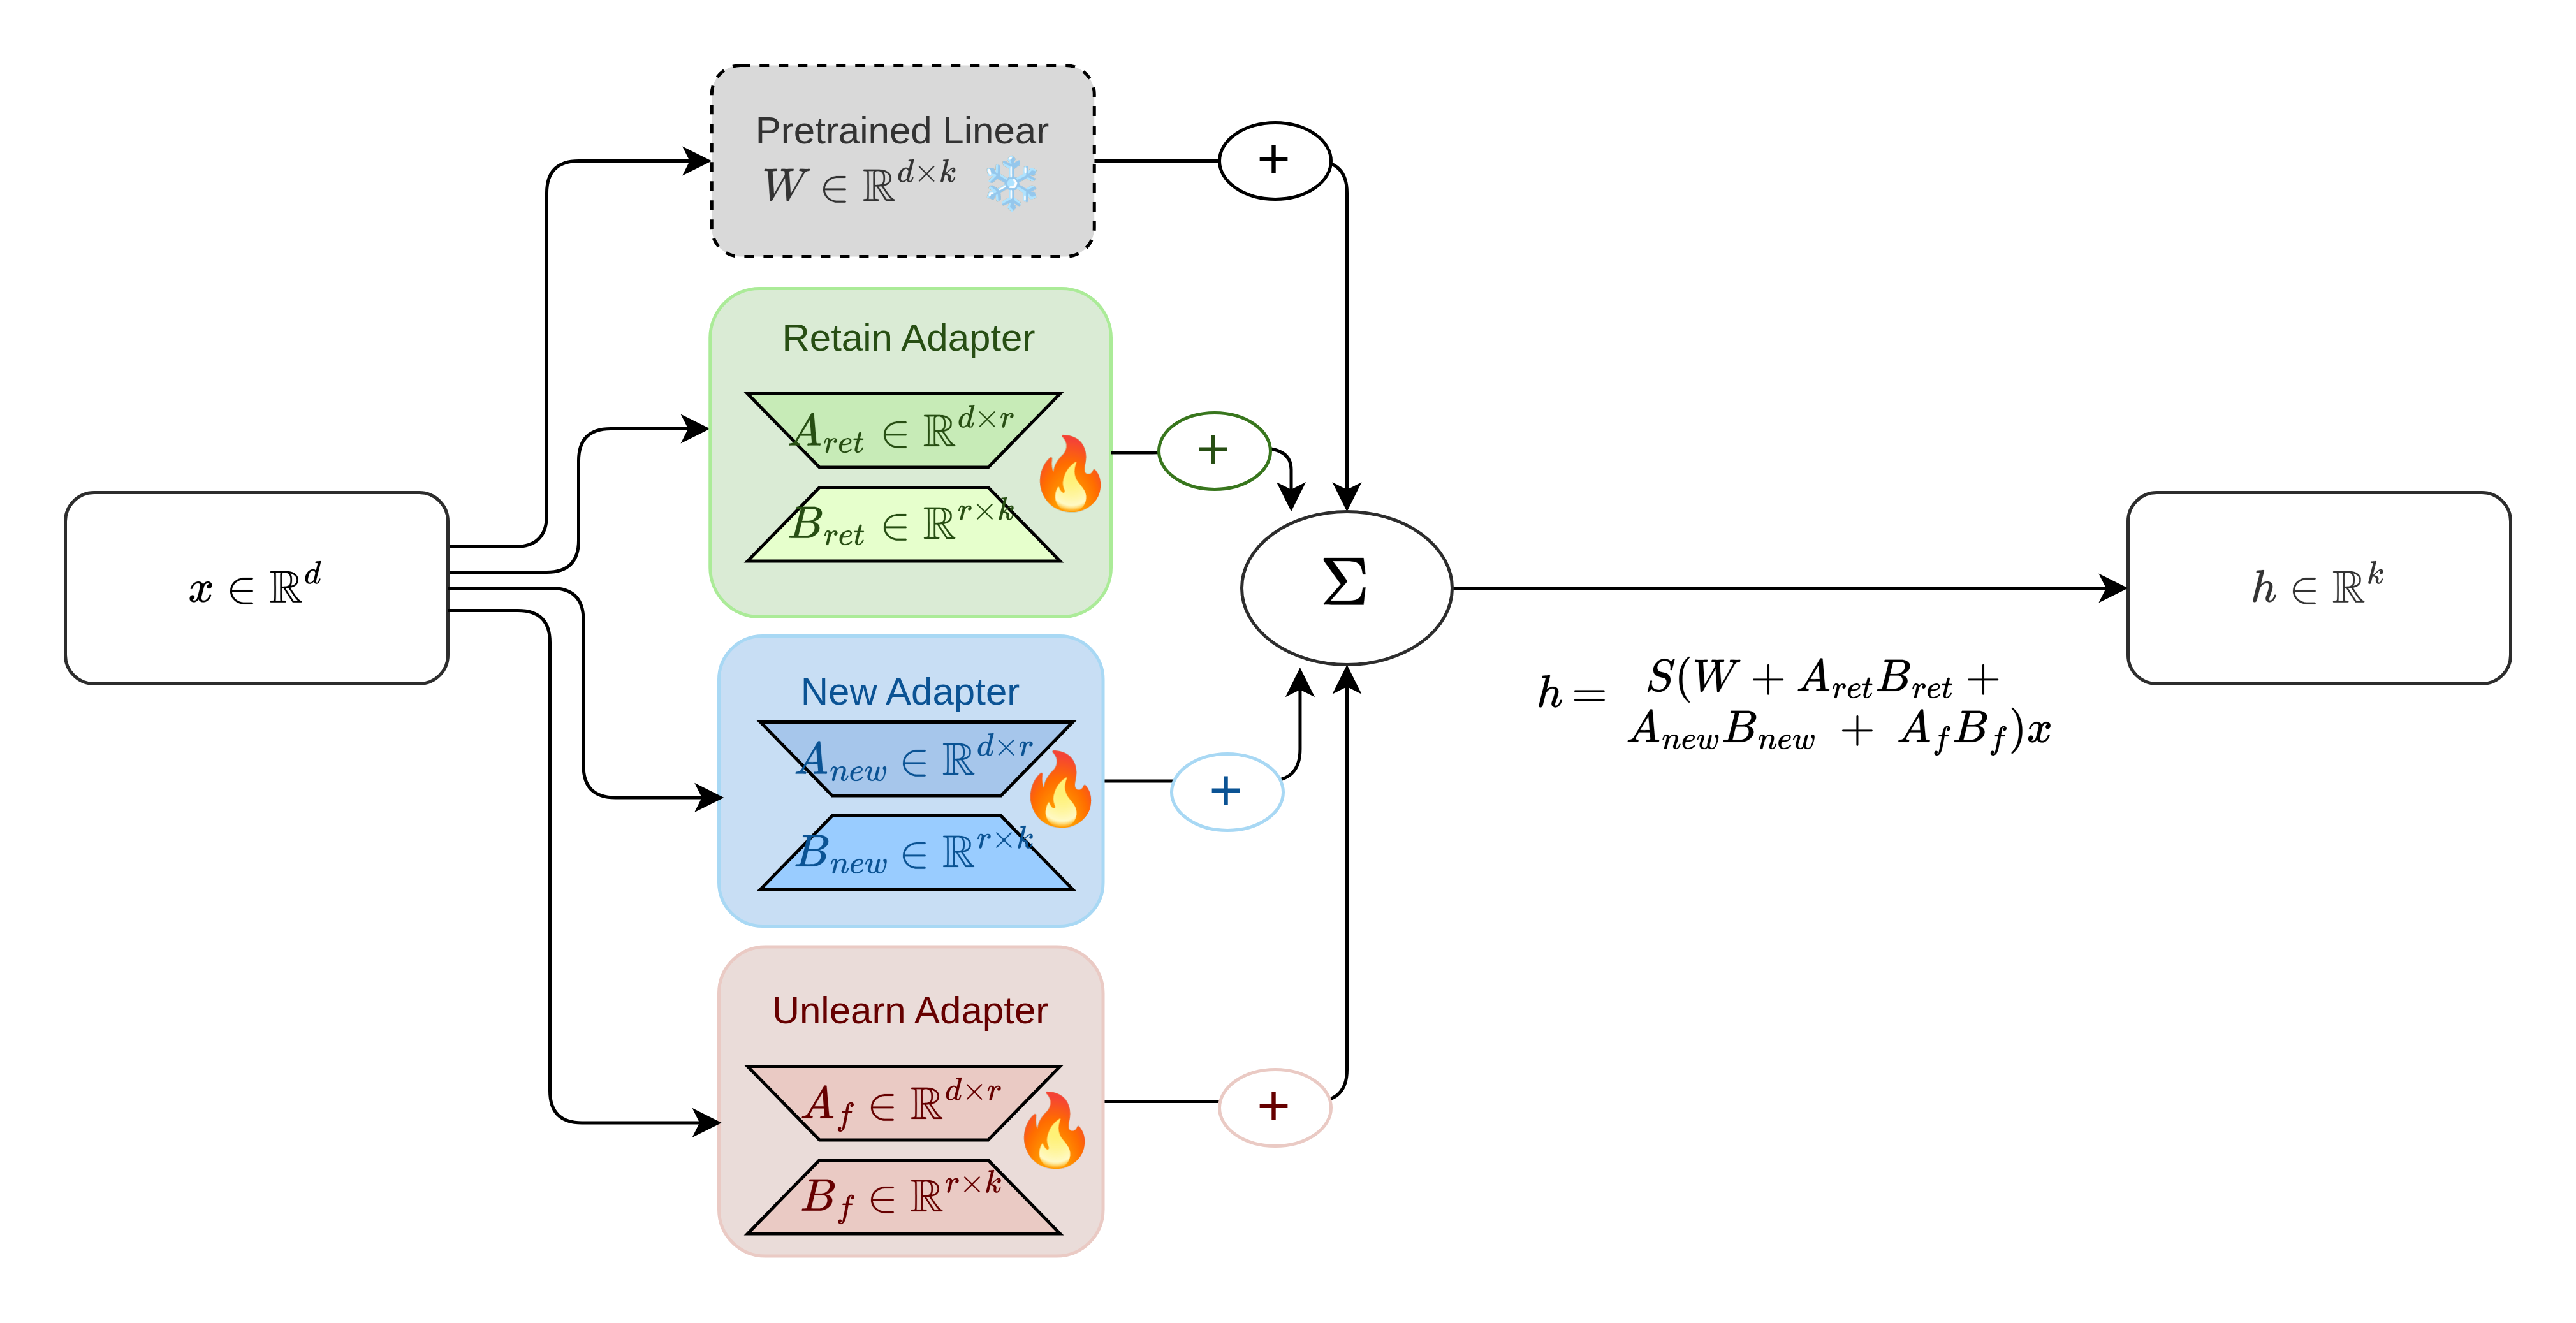
\includegraphics[width=0.75\linewidth]{images/pathwayas2.png}
    % \caption{Pathway separation for BID-LoRA, where \emoji{fire} indicates trainable and \emoji{snowflake} indicates frozen.}
    \caption{Pathway separation for BID-LoRA.}
    \label{fig:path_way_sepration}
\end{figure}

\begin{equation}
c_k = \frac{1}{|D_k|}\sum_{x \in D_k} \text{emb}(x)
\end{equation}

This yields retain centroids $\{c_{r_1}, c_{r_2}, \dots, c_{r_K}\}$ and forget centroids $\{c_{f_1}, c_{f_2}, \dots, c_{f_M}\}$. We obtain the escape direction by solving the minimax problem:
\begin{equation}
\mathbf{d}^* = \arg\min_{\|\mathbf{d}\|=1} \max_{i} \left( \mathbf{d}^\top c_{r_i} \right)
\end{equation}

where $\mathbf{d}^* \in \mathbb{R}^{\text{\textit{dim}}}$ is the escape direction vector in the $\textit{dim}$-dimensional embedding space, $\mathbf{d}^\top$ denotes the transpose, and $\mathbf{d}^\top c_{r_i}$ computes the dot product measuring the projection of retain centroid $c_{r_i}$ along direction $\mathbf{d}$. The constraint $\|\mathbf{d}\|=1$ ensures unit norm. The inner $\max_i$ identifies the retain centroid most aligned with $\mathbf{d}$, while the outer $\min$ searches over all unit directions to find $\mathbf{d}^*$ that minimizes this maximum alignment. Starting from a randomly initialized direction, the optimization iteratively converges to $\mathbf{d}^*$, yielding the direction maximally distant from all retain centroids.

\textcolor{red}{The forget adapter does not assign forgotten samples to another class. It pushes their embeddings toward a single escape point, computed via the minimax objective above to be equally far from every retain class centroid, rather than close to any one of them. Since the target is a point in embedding space and not a class label, the mechanism has no notion of a preferred wrong class to route samples toward. This distinguishes escape unlearning from systematic relabeling, where a model would be trained to consistently output one specific incorrect label (see Section~\ref{7.7} for the empirical Sink measurement that verifies this).}

However, placing the escape point on the unit sphere leads to unstable forgetting (see Section~\ref{7.6}). Therefore, we scale the escape point away from the sphere:

\begin{equation}
\mathbf{t}_{\text{escape}} = \lambda_{\text{esc}} \cdot \mathbf{d}^*
\end{equation}

This provides a target location away from retain embeddings in both direction and distance. The forget loss is then:
\begin{equation}
\mathcal{L}_{\text{\textit{f}}} = \text{MSE}\left( \text{emb}(\mathbf{X}^f), \mathbf{t}_{\text{escape}} \right)
\end{equation}

Where \text{MSE} indicates mean squared loss while this $\mathcal{L}_{\text{\textit{f}}}$ pushes all forget sample embeddings toward the escape point, creating a many-to-one mapping that destroys class-discriminative information.

\medskip
\noindent
\textit{Retention Loss}
The retention loss preserves knowledge of retain classes and prevents model drift toward the escape point through two complementary terms:
\begin{equation}
\mathcal{L}_{\text{\textit{ret}}} = \lambda_{\text{ce}} \cdot \text{CE}(\mathbf{z}_r, y_r) + \lambda_{\text{emb}} \cdot \text{MSE}(\mathbf{e}_r, \mathbf{e}_t)
\end{equation}

where $\mathbf{z}_r$ are student logits for retain samples, $y_r$ are ground truth labels, and $\mathbf{e}_r$, $\mathbf{e}_t$ are student and teacher embeddings respectively. The embedding anchor term $\text{MSE}(\mathbf{e}_r, \mathbf{e}_t)$ prevents representation drift by keeping student embeddings close to the teacher (i.e., away from escape point \textcolor{red}{$\mathbf{t}_{\text{escape}}$}), where the teacher is a frozen copy of the model at initialization.

\medskip
\noindent
\textit{New Knowledge Loss}
The model must simultaneously learn new classes using standard cross-entropy:
\begin{equation}
\mathcal{L}_{\text{\textit{new}}} = \text{CE}(\mathbf{z}_n, y_n)
\end{equation}

where \text{CE} indicates cross entropy loss $\mathbf{z}_n$ are logits and $y_n$ are labels for new class samples. 

\textcolor{red}{Although the three adapter outputs sum into the shared activation $h$ (Eq.~\ref{eq:merge}) during the forward pass, we isolate optimization at the parameter level: non-target adapters are frozen during each loss's backward pass, so gradients are never applied to their weights even though the forward computation is shared. Consequently each loss updates only its designated adapter and corresponding classifier-head nodes, without altering the other two pathways.} During gradient updates, non-target adapters are frozen and non-target head gradients are masked to zero. Specifically, $\mathcal{L}_{\text{\textit{f}}}$, $\mathcal{L}_{\text{\textit{ret}}}$, and $\mathcal{L}_{\text{\textit{new}}}$ update only their respective adapters $(B, A)$ and corresponding classifier head nodes. This ensures forgetting cannot corrupt retained knowledge and each adapter specializes to its function, as per assumption~2 (Section~\ref{3.2}), if only learning or unlearning is required, the corresponding loss terms are masked accordingly.

\textcolor{red}{
\noindent\textbf{Classifier-head handling.}
The classification head is a single linear layer with one output node per class, incrementally extended whenever new classes are introduced. At each step $t$, its nodes are partitioned into retain-, forget-, and new-class subsets; the masking scheme described above (non-target gradients masked to zero) applies identically to the head, so a given loss updates only its corresponding subset of head nodes. At the following step, nodes that were new-class at step $t$ are reclassified as retain-class nodes, while forgotten nodes from step $t$ remain excluded going forward. After merging, we remove the head's forget-class output nodes entirely, consistent with the adapter-deletion rationale of Assumption~4 (Section~\ref{3.2}): since escape unlearning collapses forget-class embeddings to a single point, their corresponding head weights carry no discriminative signal, and retaining them would needlessly expose which classes were removed.
}

\textcolor{red}{
\noindent\textbf{Why adapter deletion is necessary.}
After merging, the adapted model satisfies $\mathcal{M}' = \mathcal{M}_\text{orig} \oplus \mathcal{S}(B_\text{ret}A_\text{ret} + B_\text{new}A_\text{new} + B_f A_f)$. If all adapter matrices are retained, an adversary can exactly reconstruct the pre-adaptation model as shown below
\begin{equation}
\mathcal{M}_\text{orig} = \mathcal{M}' \ominus \mathcal{S}\!\left(B_\text{ret}A_\text{ret} + B_\text{new}A_\text{new} + B_f A_f\right),
\label{eq:recovery}
\end{equation}
fully recovering all unlearned knowledge. Permanent deletion of adapter matrices and $\mathcal{M}_\text{orig}$ post-merge eliminates this inversion, making recovery computationally intractable (Assumption~4, Section~\ref{3.2}).
}

\label{4.4}
Algorithm~\ref{alg:bidlora} summarizes the complete BID-LoRA training procedure. Each iteration performs gradient-isolated updates for retain, forget, and new pathways sequentially, ensuring no cross-pathway interference. After training, adapters merge into base weights for efficient inference. \textcolor{red}{Delete all adapters post-merge (Assumption~4).}
\begin{algorithm}[!htbp]
\caption{BID-LoRA Training}
\label{alg:bidlora} 
\begin{algorithmic}[1]
\Require Pre-trained model $\mathcal{M}$, retain data $D^\text{\textit{full}}_r$, forget data $D_f$, new data $D_\text{\textit{new}}$, replay buffer $D_r$ 
and $\mathcal{S}$ be the LoRA scaling factor
\Ensure Updated model with merged adapters

\State Initialize adapters $(B_{\text{\textit{ret}}}, A_{\text{\textit{ret}}})$, $(B_{\text{\textit{new}}}, A_{\text{\textit{new}}})$, $(B_{\text{\textit{f}}}, A_{\text{\textit{f}}})$
\State Freeze backbone weights $W$
\State $\mathcal{M_\text{\textit{t}}} \gets \text{copy}(\mathcal{M})$ \Comment{Frozen teacher for embedding anchor}

\State \textbf{// Compute escape point}
\For{each class $k$ in $D_r$}
    \State $c_k \gets \frac{1}{|D_k|}\sum_{x \in D_k} \text{emb}(x)$ \Comment{Retain centroids}
\EndFor
\State $\mathbf{d}^* \gets \arg\min_{\|\mathbf{d}\|=1} \max_{i} (\mathbf{d}^\top c_{r_i})$ \Comment{Escape direction}
\State $\mathbf{t}_{\text{escape}} \gets \lambda_{\text{esc}} \cdot \mathbf{d}^*$ \Comment{Escape point}

\For{epoch $= 1$ to $E$}
    % \For{each mini-batch $(X_\text{\textit{ret}}, X_\text{\textit{f}}, X_\text{\textit{new}})$}
    \For{each mini-batch $(X_\textit{ret}, y_\textit{ret}), (X_f, y_f), (X_\textit{new}, y_\textit{new})$ from $(D_r, D_f, D_\textit{new})$}
        \State \textbf{// Retention update}
        \State Freeze $(B_{\text{f}}, A_{\text{f}})$, $(B_{\text{new}}, A_{\text{new}})$
        \State $\mathbf{z}_\text{\textit{ret}} \gets \mathcal{M}(X_\text{\textit{ret}})$ \Comment{Student logits}
        \State $\mathbf{e}_\text{\textit{ret}} \gets \text{emb}(X_\text{\textit{ret}})$ \Comment{Student embeddings}
        \State $\mathbf{e}_\textit{ret,t} \gets \mathcal{M}_t.\text{emb}(X_\text{\textit{ret}})$ \Comment{Teacher embeddings}
        \State $\mathcal{L}_{\text{ret}} \gets \lambda_{\text{ce}} \cdot \text{CE}(\mathbf{z}_\textit{ret}, y_\textit{ret}) + \lambda_{\text{emb}} \cdot \text{MSE}(\mathbf{e}_\textit{ret}, \mathbf{e}_\textit{t,ret})$
        \State Update $(B_{\text{ret}}, A_{\text{ret}})$ and retain-class head
        
        \State \textbf{// Forget update}
        \State Freeze $(B_{\text{\textit{ret}}}, A_{\text{\textit{ret}}})$, $(B_{\text{\textit{new}}}, A_{\text{\textit{new}}})$
        \State $\mathcal{L}_{\text{forget}} \gets \text{MSE}(\text{emb}(X_\text{\textit{f}}), \mathbf{t}_{\text{escape}})$
        \State Update $(B_{\text{\textit{f}}}, A_{\text{\textit{f}}})$ and forget-class head
        
        \State \textbf{// New knowledge update}
        \State Freeze $(B_{\text{\textit{ret}}}, A_{\text{\textit{ret}}})$, $(B_{\text{\textit{f}}}, A_{\text{\textit{f}}})$
        \State $\mathcal{L}_{\text{\textit{new}}} \gets \text{CE}(\mathcal{M}(X_\text{\textit{new}}), y_n)$
        \State Update $(B_{\text{\textit{new}}}, A_{\text{\textit{new}}})$ and new-class head
    \EndFor
\EndFor

\State \textbf{// Merge adapters}
\State \textcolor{red}{$W \gets W + \mathcal{S}(B_{\text{\textit{ret}}}A_{\text{\textit{ret}}} + B_{\text{\textit{new}}}A_{\text{\textit{new}}} + B_{\text{\textit{f}}}A_{\text{\textit{f}}})$}
\State \textcolor{red}{\textbf{Delete} $(B_f, A_f)$, $(B_\text{\textit{ret}}, A_\text{\textit{ret}})$, $(B_\text{\textit{new}}, A_\text{\textit{new}})$, pre-adaptation checkpoint $\mathcal{M}_\text{orig}$, and forget-class head nodes}

\State \Return $\mathcal{M}$
\end{algorithmic}
\end{algorithm}
